\textbf{Ejemplo 7}\\
Una industria puede adquirir una máquina a un costo de  COP  6.000.000, tendrá una vida útil de 5 años y prácticamente no tendrá valor de salvamento, la máquina será totalmente depreciada en 3 años por partes iguales, el estudio de mercados indica que los ingresos del primer año serán aproximadamente de  COP  3.000.000 y aumentarán todos los años un 30\% periodo año vencido, por otra parte, se estima que el costo de producción del primer año será de  COP  800.000 y cada año aumentará en  COP  200.000. Suponiendo una tasa impositiva del 38\% nominal anual año vencido. Determinar la rentabilidad del proyecto usando un horizonte de planeación de 5 años.
\\

\textbf{Solución.}\\
%La tabla ira centrada
\begin{center}
	\renewcommand{\arraystretch}{1.5}% Margenes de las celdas
	%Creación de la cuadricula de 3 columnas
\begin{longtable}[H]{|c|c|c|}
		%Creamos una linea horizontal
\hline
		%Definimos el color de la primera fila
\rowcolor[HTML]{FFB183}
%%%%% INICIO ASIGNACIÓN PERÍODO FOCAL %%%%%%%
  %%%%%%%%%% INICIO TITULO
  %Lo que se hace aquí es mezclar las 3 columnas en una sola
  \multicolumn{3}{|c|}{\cellcolor[HTML]{FFB183}\textbf{1. Asignación período focal}}   \\ \hline
  %%%%%%%%%% FIN TITULO
  %%%%% INICIO DECLARACIÓN DE VARIABLES %%%%%%%
  \multicolumn{3}{|c|}{$pf = No Aplica$}   \\ \hline
  
%%%%%%%%%%% INICIO TITULO
\rowcolor[HTML]{FFB183}
\multicolumn{3}{|c|}{\cellcolor[HTML]{FFB183}\textbf{2. Declaración de variables}}    \\ \hline
%%%%%%%%%%% FIN TITULO
%%%%%%%%%%% INICIO MATEMÁTICAS
\multicolumn{3}{|c|}{$ VPN= COP  ?$}  
\\

\hline

		%%%%%%%%%%%%% FIN INSERCIÓN DE IMAGEN
		%%%%%FIN FLUJO DE CAJA
		
		
		
		%%%%% INICIO DECLARACIÓN FORMULAS
		%%%%%%%%%%% INICIO TITULO
\rowcolor[HTML]{FFB183}
\multicolumn{3}{|c|}{\cellcolor[HTML]{FFB183}\textbf{3. Declaración de fórmulas}}    \\ \hline
		%%%%%%%%%%% FIN TITULO
		%%%%%%%%%%% INICIO MATEMÁTICAS
\multicolumn{3}{|c|} {$ \text{Base = Ingreso — Costo — Depreciación.} $}   \\ 
\multicolumn{3}{|c|} {$ \text{Impuesto = 0.38 x Base} $}   \\ 
\multicolumn{3}{|c|} {$ \text{FNC = Ingreso — Costo — Impuesto} $}   \\
\hline	
	
		%%%%%%%%%% FIN MATEMÁTICAS
		%%%%%% INICIO DESARROLLO MATEMÁTICO
\rowcolor[HTML]{FFB183}
		%%%%%%%%%%INICIO TITULO
\multicolumn{3}{|c|}{\cellcolor[HTML]{FFB183}\textbf{4. Desarrollo matemático}}       \\ \hline
		%%%%%%%%%% FIN TITULO
		%%%%%%%%%% INICIO MATEMÁTICAS
		\multicolumn{3}{|c|}{$ \text{A continuación presentamos la tabla necesaria para calcular el flujo de caja.} $}  
		\\
		\multicolumn{3}{|c|}{ 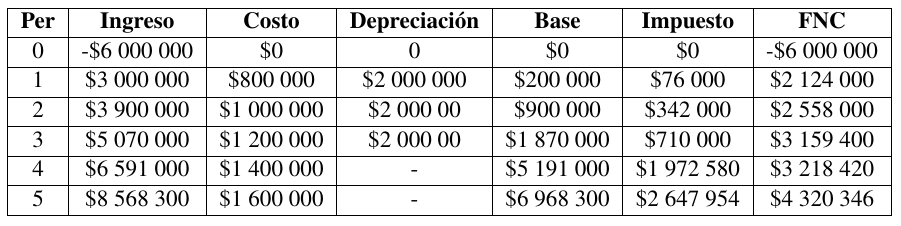
\includegraphics[scale=0.6, trim=-5 -5 -5 -5]{tabla_ejemplo_8.png} }   
		\\ 
		\multicolumn{3}{|c|}{$ \text{Si hacemos el VPN=0 podemos hallar la TIR.} $}  
		\\
		\multicolumn{3}{|c|}{$VPN = -  COP  6.000.000 +  COP  2.124.000(1+i)^{-1} +  COP  2.558.000(1+i)^{-2} $}  
		\\
		\multicolumn{3}{|c|}{$ +  COP  3.159.400(1+i)^{-3} +  COP  3.218.420(1+i)^{-4} +  COP  4.320.346(1+i)^{-5} =  COP 0 $}  
		\\
		\multicolumn{3}{|c|}{$ \text{Al resolver esta ecuación por interpolación se obtiene:} $}  
		\\
		\multicolumn{3}{|c|}{$ \text{i = 36.58\% naav} $}  
		\\ 	
	    \hline
				
		%%%%%%%%%% FIN MATEMÁTICAS
		%%%%%% FIN DESARROLLO MATEMÁTICO
		%%%%%% INICIO RESPUESTA
\rowcolor[HTML]{FFB183}
		%%%%%%%%%%INICIO TITULO
\multicolumn{3}{|c|}{\cellcolor[HTML]{FFB183}\textbf{5. Respuesta}}   \\ \hline
		%%%%%%%%%% FIN TITULO
		%%%%%%%%%% INICIO RESPUESTA MATEMÁTICA
		
\multicolumn{3}{|c|}{ \text{i = 36.58\% naav que viene a ser la rentabilidad del proyecto.}}
\\
\hline

		
		%%%%%%%%%% FIN MATEMÁTICAS
		%%%%%% FIN RESPUESTA
	\end{longtable}
	%Se crean dos lineas en blanco para que no quede el siguiente texto tan pegado
	%\newline \newline %USARLO SI CREES QUE ES NECESARIO
\end{center}
%%%%%%%%%%%%%%%%%%%%%%%%%%FIN EJERCICIO 1 %%%%%%%%%%%%%%%%%%%%%%%%%%%


\textbf{}\\
